\documentclass[openright,twoside,headsepline]{scrbook}
\usepackage{graphicx}
\usepackage[applemac]{inputenc}
\usepackage{amsmath,amssymb,amsfonts,amsthm}
\begin{document}
\graphicspath{{/Users/lentz/Documents/GitHub_locals/Thesis/images/}}



\chapter{Theory}

\section{Models of infectious diseases}
%\subsection{Observations}
\paragraph{Observations:} Large scale patterns of epidemics have been measured \cite{geissel_der_menschheit}
The spread of infectious diseases is something that everyone is familiar with.

\paragraph{The science inspired by observation.} One goal of epidemiology is to understand the principles behind the spreading process, i.e. the way how a disease is transmitted through a population.
In this context, \emph{conceptional} models are used.
They make use of simple assumptions for the local (person-to-person) dynamics and focus on the big picture of the process.
Conceptual models are very similar to models in theoretical physics, because they focus on the very essence of the problem (here: the macroscopic view, spreading patterns).
However, they have to neglect many details of the real problem (here: physiology, symptoms, individual behavior, infection pathways and many more!).

Another important issue of epidemiology is the \emph{forecast} of epidemic spreading processes.
Forecast models incorporate as much information as possible and the main focus is not an understanding of the basic principles.

This section summarizes the mathematical framework that roughly reproduces the behavior of some infectious diseases and briefly discusses some important insights.


\subsection{Development}



\subsection{Infection dynamics}

The spread of infectious diseases can be modeled in terms of compartment models as described in section xx.
We differentiate between \emph{conceptional models} and \emph{realistic disease models}.
While the former class is used to provide conceptual results as for the computation of thresholds or to test theories \cite{Hethcote:2000}, realistic disease models use as many aspects as possible to provide a forecast of the spreading process.
Realistic disease models can be very complex and are beyond the scope of this work, thus the author focuses on the use of conceptional models.
The following section is inspired by the Lecture notes of J.~R.~Chasnov \cite{Chasnov:2010}.

\subsection{SI model}\label{sec:si_model}
Let us consider a population of $N$ individuals.
In the simplest case, the infection status of each individual is either susceptible or infected and there are no births and deaths on the population.
Susceptible individuals become infected, if they are in contact with an infected.
This mimics the behavior of an infectious disease without immunization, i.e. infected individuals stay permanently infected.

Provided that $\alpha $ is the rate, under which new susceptible become infected, the SI-model is as follows:
\begin{align}\label{eq:si_model}
\frac{dS}{dt} &= -\alpha SI \nonumber \\
\frac{dI}{dt} &= \alpha SI,
\end{align}
where $S$ and $I$ are the numbers of susceptible and infected individuals respectively.
The total population is $N=S+I$.
Thus, \eqref{eq:si_model} can be rewritten as
$$
\frac{dI}{dt}=\alpha (N-I)I,
$$
i.e. a logistic differential equation.
Hence, in the limit $t\rightarrow \infty $ the whole population is infected ($I(\infty )=N$). 

\subsection{SIR model}\label{sec:sir_model}
In contrast of the infection dynamics introduced in the previous section, many epidemics allow for an immunization of the individuals.
Examples are measles or whooping cough \cite{grenfell:92} \cite{andersonmay:92}.
In this case, individuals recover from the disease after being infected for a certain time period.
The infection scheme has to be extended to susceptible-infected-recovered (SIR) as in the following infection model \cite{kermack:27}:
\begin{align}\label{eq:sir_model}
\frac{dS}{dt} &= -\alpha SI \nonumber \\
\frac{dI}{dt} &= \alpha SI -\gamma I \nonumber \\
\frac{dR}{dt} &= \gamma I
\end{align}
where $\alpha $ is the infection rate and $\gamma $ is the immunization or recovery rate.
There is no analytic solution for the system \eqref{eq:sir_model}, but some fundamental conclusions can be obtained analytically.
We show a typical solution of \eqref{eq:sir_model} in figure \ref{fig:std_sir_model}.
%
\begin{figure}[htbp]
\begin{center}
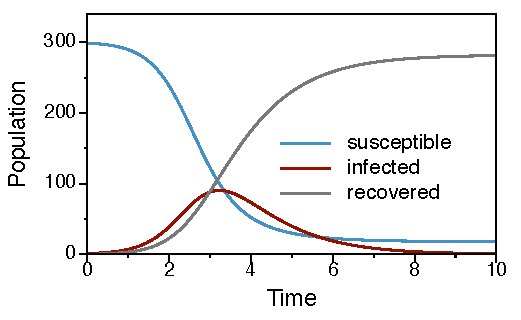
\includegraphics{sir_model.pdf}
\caption{Typical solution of a susceptible-infected-recovered (SIR) model. Parameters: $\alpha = 3$, $\gamma = 1$, $N=300$, $S_0=1$.}
\label{fig:std_sir_model}
\end{center}
\end{figure}
%

The SIR model shows more sophisticated features than the SI model \eqref{eq:si_model}.
To begin with, we analyze the fixed points of the system, i.e. $(S_*,I_*,R_*)$ where
\begin{equation}
\frac{dS_*}{dt} = -\alpha S_*I_* =0 ,\; \;\;
\frac{dI_*}{dt} = \alpha S_*I_* -\gamma I_* =0,\; \;\;
\frac{dR_*}{dt} = \gamma I_* = 0.
\end{equation}
It follows from the last equation that $I_*=0$ at the fixed point, where $S_*$ and $R_*$ can be arbitrary.
Hence, a fixed point is $(S_*,0,R_*)$.

Let us analyze the stability of the fixed point in the early phase of an infection.
Almost all individuals are susceptible and consequently $I_*=N-S_*$.
An outbreak occurs, if and only if $dI/dt >0$ in this phase, i.e.
\begin{equation}\label{eq:prelim_condition}
\frac{dI}{dt}=\alpha S_* (N-S_*) - \gamma (N-S_*)=(N-S_*)(\alpha S_* -\gamma ) >0.
\end{equation}
It follows from \eqref{eq:prelim_condition} that the number of infected grows, if
\begin{equation}\label{eq:prelim_rnod}
\alpha S_* / \gamma >1.
\end{equation}
Equation \eqref{eq:prelim_rnod} is extremely important in epidemiology, because it defines a threshold for the unfolding of an infection spreading process.
We call this fraction the \emph{basic reproduction number} $R_0$.
Recall that $S_* \approx N$ in the fixed point.
Thus it follows that the outbreak condition is
\begin{equation} \label{eq:r0}
R_0 = N \frac{\alpha }{\gamma } >1.
\end{equation}

The basic reproduction number describes the average number of follow-up infections by each infected individual.
It is one of the main goals in epidemiology to bring down the basic reproduction number of a disease below the critical value $R_0=1$.
This is the reason for the implementation of mass vaccination.
As one can immediately see from equation \eqref{eq:r0}, this can be done by reducing the infection rate $\alpha $ or by increasing the immunization rate $\gamma $.
In principle, one could also reduce the size of the initial population $S_*$.
As an example, reducing the infection rate can be done by increasing hygiene standards or appropriate behavior, say wearing warm clothes in winter time to avoid common cold.
The immunization rate can be increased by vaccination.

Let us now focus on the late phase of an SIR-infection.
In contrast to the SI-model of section \ref{sec:si_model} an SIR like outbreak does not necessarily infect the whole population, even if $R_0>1$.
The reason is that there has to be a critical mass of susceptible individuals in order to keep an infection alive (see equation \eqref{eq:prelim_rnod}).
The total number of infected during an infection given by the number of recovered at the end of the infection, since every recovered has to be in the infected state in the first place.
A central measure throughout this work is therefore the \emph{outbreak size} $R_\infty$.

To compute the outbreak size, we consider the second fixed point of \eqref{eq:sir_model}, i.e. the fixed point for $t \rightarrow \infty $.
At this point there are no infected and a fraction of the population is recovered.
Hence the fixed point is $(N-R_\infty , 0, R_\infty )$.
A simple way to obtain the outbreak size $R_\infty $ is to use equations \eqref{eq:sir_model} and compute 
$$
\frac{dS}{dR}=-\frac{\alpha }{\gamma } S 
$$
and separate the variables \cite{Chasnov:2010}.
This yields
$$
\int _{S_*} ^{N-R_\infty} \frac{dS}{S}=-\frac{\alpha }{\gamma } \int _{R_*} ^{R_\infty} dR .
$$
We integrate from the initial condition at $t=0$ to the final condition at $t \rightarrow \infty$, where $S_\infty = N-R_\infty $.
Using that $R_* =0$ at $t=0$ gives 
\begin{equation}\label{eq:transcendental}
R_\infty = S_*-S_* e ^{-\frac{\alpha}{\gamma}R_\infty}.
\end{equation}
This transcendental equation can be solved numerically using a Newton-Raphson technique.
The outbreak size $R_\infty $ only takes finite values for $\alpha / \gamma > 1$.
A solution of equation \eqref{eq:transcendental} is shown in figure \ref{fig:transcendental}
%
\begin{figure}[htbp]
\begin{center}
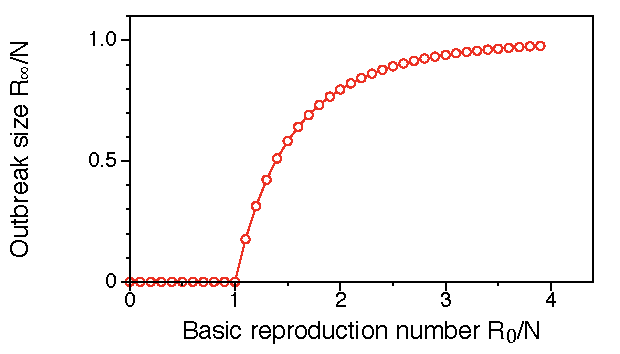
\includegraphics{R_0_R_infty.pdf}
\caption{Relative outbreak size vs. basic reproduction number.
The outbreak size takes finite values only for $R_0/N >1$.
Note that even for supercritical $R_0$ the outbreak size is in general smaller than the total population.
}
\label{fig:transcendental}
\end{center}
\end{figure}

It should be noted that an SIR epidemic is a single event, i.e. it possesses a \emph{characteristic time scale}.
The analysis of the late phase of an epidemic also gives information about these time scales.
Let us consider the second equation of \eqref{eq:sir_model}.
\begin{equation}\label{eq:sir_model_only_i}
\frac{dI}{dt} = \alpha SI -\gamma I
\end{equation}
In the late phase of an SIR-type epidemic, the fraction of infected is small.
Given sufficiently large values of $R_0$, the fraction of recovered is also small in this phase (see figure \ref{fig:transcendental}).
Thus, we neglect the quadratic term in \eqref{eq:sir_model_only_i}.
This gives $\frac{dI}{dt} = -\gamma I $, which has the solution
$$
I(t)=I(0)e^{-\gamma t}.
$$
Hence, the infection decays exponentially for large $t$ and the inverse recovery rate $1/\gamma $ defines the characteristic time of the epidemic.

\subsection{Force of infection}
The model presented in section \ref{sec:sir_model} describes only the very basic behavior of epidemic dynamics, and is therefore a conceptual model.
However, it is one of the main objectives in epidemiology to have an understanding of the exact infection rates in the process.
Infection rates their selves can cause complex infection dynamics.

The term $\alpha I$ used in section \ref{sec:sir_model} is a special, very simple case of an infection rate.
More generally, we have to replace $\alpha I$ by an abstract infection rate $\lambda $ containing more information about the interaction between susceptible and infected individuals \cite{Keeling:2005}.
Thus, the equation for the infected becomes
$$
dI/dt = -\lambda S -\gamma I.
$$
The rate $\lambda $ is called the \emph{force of infection}.
In principle, this parameter can be arbitrarily complex, because it contains detailed information about the mixing properties of the population.
This information could be given as contact networks, demographic contact structures, etc.

In most cases, detailed information about mixing is not available.
Instead, we assume \emph{random mixing} of the population, i.e. every individual can be in contact with every other individual.
This yields a transmission rate \cite{Keeling:2005}
\begin{equation}\label{eq:force_of_infection}
\lambda = \tau n \frac{I}{N}\equiv \beta \frac{I}{N},
\end{equation}
where $\tau $ is the transmission rate, $n$ is the effective contact rate and $I/N$ is the fraction of infectious contacts.
It is therefore reasonable to replace the infection term $\alpha $ in \eqref{eq:sir_model} by $\beta /N$ to explicitly include the force of infection.
Nevertheless, the results presented in section \ref{sec:sir_model} remain qualitatively the same.

Although the force of infection gives a more reasonable description of the infection process, the assumption of random mixing remains inappropriate for many real world systems.
Due to the availability of contact data, the random mixing assumption can be improved in terms of contact networks.
Even if the exact data of an epidemic system is not available, research on complex networks allows us to give more realistic models about mixing.
In the next section, we briefly report important results in complex network research and focus on the interplay between networks and epidemics in section \ref{sec:epidemics_on_networks}.


\section{Complex networks}


\section{Epidemics on networks}\label{sec:epidemics_on_networks}
\subsection{From random mixing to developed structure}

\end{document}
